\documentclass{beamer}
\setbeamerfont{subsection in toc}{size=\footnotesize}
%\setbeameroption{show notes on second screen=left} %enable for notes
\usepackage{graphicx}
\usepackage{xcolor}
\usepackage{listings}
\usepackage{hyperref}
\lstset{language=python,frame=single}
\usepackage{verbatim}
\usepackage[longnamesfirst]{natbib}
\usepackage{subcaption}
\usepackage{amsmath}
\usepackage{bm}
\usepackage{relsize}
\usepackage{appendixnumberbeamer}
\usepackage{xparse}
\usepackage{multimedia}
\usepackage{xcolor}
\usepackage[normalem]{ulem}
\usepackage{hyperref}
\usepackage{tikz}
\usetikzlibrary{matrix,backgrounds}
\usetikzlibrary{positioning}
\usetikzlibrary{shapes,arrows}
\usetikzlibrary{positioning}

\captionsetup[subfigure]{labelformat=empty}

\tikzset{onslide/.code args={<#1>#2}{%
  \only<#1>{\pgfkeysalso{#2}} 
}}

\tikzstyle{block} = [rectangle, draw, thick, align=center, rounded corners]
\tikzstyle{boundingbox} = [thick, lightgray]
\tikzstyle{dashblock} = [rectangle, draw, thick, align=center, dashed]
\tikzstyle{conc} = [ellipse, draw, thick, dashed, align=center]
\tikzstyle{netnode} = [circle, draw, very thick, inner sep=0pt, minimum size=0.5cm]
\tikzstyle{relunode} = [rectangle, draw, very thick, inner sep=0pt, minimum size=0.5cm]
\tikzstyle{line} = [draw, very thick, -latex', -]
\tikzstyle{arrow} = [draw, ->, very thick]

\definecolor{bpurp}{HTML}{984ea3}
\definecolor{bblue}{HTML}{377eb8}

\usetheme[numbering=none]{metropolis}

\begin{document}

\title{Meta-Mapping: Toward human-like flexibility from deep learning}
\author{Andrew Lampinen}
\date{}
\frame{\titlepage}

\begin{frame}{Humans are good at adapting flexibly}
\centering
\includegraphics[width=\textwidth]{figures/poker.png}
\end{frame}

\begin{frame}{Deep learning is (usually) not}
\begin{columns}
\begin{column}{0.5\textwidth}
Deep learning generally requires lots of data to achieve good performance on a task.\uncover<2->{ However, there are a few exceptions:}
\begin{itemize}
    \item<3-> Lots of new work on meta-learning (learning to learn), for learning from little data, but not none.
    \item<4-> Some language work I'll come back to later.
\end{itemize}
\end{column}

\begin{column}{0.5\textwidth}
\includegraphics[width=\textwidth]{figures/frostbite.jpg}
\end{column}
\end{columns}
\end{frame}

\begin{frame}[standout]
How can we build deep learning models that can perform a new task on their first try?
\end{frame}

\section{Meta-mapping}

\begin{frame}{Tasks as functions}
\begin{columns}
\begin{column}{0.5\textwidth}
It's useful to think of tasks or behaviors as functions mapping input to output:
\begin{itemize}
    \item Poker hand \(\rightarrow\) bet
    \item Chess position \(\rightarrow\) move
    \item Object \(\rightarrow\) classification
\end{itemize}
Standard deep learning tries to infer this function from lots of examples. 
\end{column}

\begin{column}{0.5\textwidth}
\includegraphics[width=\textwidth]{figures/poker_function.png}
\end{column}
\end{columns}
\end{frame}

\begin{frame}{Meta-learning}
\begin{columns}
\begin{column}{0.5\textwidth}

\begin{itemize}
    \item Lots of recent research on meta-learning -- learning to learn.
    \item If you know a lot about card games, you should be able to pick up a new one from a few examples.
    \item Then apply this knowledge to play the game with probe hands you weren't taught. 
    \item But how could we play a variation of the game? 
\end{itemize}
\end{column}

\begin{column}{0.5\textwidth}
\includegraphics[width=\textwidth]{figures/poker_function_2.png}
\end{column}
\end{columns}
\end{frame}
%\begin{frame}[standout]
%It's useful to think of a task/behavior as a function that maps some inputs to some outputs.
%\end{frame}

\begin{frame}{Functional flexibility}
If tasks are functions, altering the task = adapting the function. 
\begin{columns}
\begin{column}{0.5\textwidth}
\vspace{2em}
\includegraphics[width=\textwidth]{figures/poker.png}
\end{column}
\begin{column}{0.5\textwidth}
\vspace{2em}
\only<1>{
\includegraphics[width=\textwidth]{figures/poker_function.png}
}
\only<2>{
\includegraphics[width=\textwidth]{figures/lose_poker_function.png}
}
\end{column}
\end{columns}
\end{frame}

\begin{frame}{Meta-mappings}
How do we get from a task function to an adapted one?
\begin{itemize}
\item We propose \textbf{meta-mappings}, higher-order functions which transform functions into other functions.
\end{itemize}
\includegraphics[width=\textwidth]{figures/meta_mapping_poker.png}
\end{frame}

\begin{frame}[standout]
We model flexibility as the ability to transform basic task functions, via a meta-mapping. 
\end{frame}

\begin{frame}{Meta-mappings are analogous to basic tasks}
\begin{columns}
\begin{column}{0.5\textwidth}
\vspace{2em}
\includegraphics[width=\textwidth]{figures/poker_function.png}
\end{column}
\begin{column}{0.5\textwidth}
\vspace{2em}
\includegraphics[width=\textwidth]{figures/try_to_lose_function.png}
\end{column}
\end{columns}
\begin{itemize}[<+->]
\item Both are just functions (they just have different types of inputs and outputs).
\item This means we can apply all the usual deep learning to learning meta-mappings.
\item ... Assuming we have a way to represent the functions as input or output. 
\end{itemize}
\end{frame}

\begin{frame}[standout]
There is a functional analogy between basic tasks and meta-mappings.
\end{frame}

\section{An architecture for representing tasks as functions}

\begin{frame}{Architecture overview}
Our goal is to implement:
\begin{itemize}
\item A way of representing tasks as functions.
\item A way of representing those tasks/functions as vectors.
\item A way of learning to transform these task-vectors to perform meta-mappings.
\end{itemize}
This will allow the architecture to perform new tasks without data, by their relationship to prior tasks.
\end{frame}

\begin{frame}{Task-specific computations are low-dimensional and abstract}
\begin{tikzpicture}[auto]
\node at (-4, 0) (image) {\includegraphics[width=2cm]{figures/straight_flush_hand.jpg}};


%% input

\node[netnode] at (-2.25, -1.5) (i00) {};
\node[netnode] at (-2.25, -0.75) (i01) {};
\node[netnode] at (-2.25, 0) (i02) {};
\node[netnode] at (-2.25, 0.75) (i03) {};
\node[netnode] at (-2.25, 1.5) (i04) {};

\path [line] ([xshift=-3]image.east) to (i00);
\path [line] ([xshift=-3]image.east) to (i01);
\path [line] ([xshift=-3]image.east) to (i02);
\path [line] ([xshift=-3]image.east) to (i03);
\path [line] ([xshift=-3]image.east) to (i04);

\node[netnode] at (-1, -1.5) (i10) {};
\node[netnode] at (-1, -0.75) (i11) {};
\node[netnode] at (-1, 0) (i12) {};
\node[netnode] at (-1, 0.75) (i13) {};
\node[netnode] at (-1, 1.5) (i14) {};

\path [line] (i00) to (i10);
\path [line] (i00) to (i11);
\path [line] (i00) to (i12);
\path [line] (i00) to (i13);
\path [line] (i00) to (i14);
\path [line] (i01) to (i10);
\path [line] (i01) to (i11);
\path [line] (i01) to (i12);
\path [line] (i01) to (i13);
\path [line] (i01) to (i14);
\path [line] (i02) to (i10);
\path [line] (i02) to (i11);
\path [line] (i02) to (i12);
\path [line] (i02) to (i13);
\path [line] (i02) to (i14);
\path [line] (i03) to (i10);
\path [line] (i03) to (i11);
\path [line] (i03) to (i12);
\path [line] (i03) to (i13);
\path [line] (i03) to (i14);
\path [line] (i04) to (i10);
\path [line] (i04) to (i11);
\path [line] (i04) to (i12);
\path [line] (i04) to (i13);
\path [line] (i04) to (i14);

%% task specific
\node[netnode] at (0.25, -0.375) (t00) {};
\node[netnode] at (0.25, 0.375) (t01) {};

\path [line] (i10) to (t00);
\path [line] (i10) to (t01);
\path [line] (i11) to (t00);
\path [line] (i11) to (t01);
\path [line] (i12) to (t00);
\path [line] (i12) to (t01);
\path [line] (i13) to (t00);
\path [line] (i13) to (t01);
\path [line] (i14) to (t00);
\path [line] (i14) to (t01);

\node[netnode] at (1.5, -0.375) (t10) {};
\node[netnode] at (1.5, 0.375) (t11) {};

\path [line] (t00) to (t10);
\path [line] (t00) to (t11);
\path [line] (t01) to (t10);
\path [line] (t01) to (t11);

%% output

\node[netnode] at (2.75, -1.5) (o00) {};
\node[netnode] at (2.75, -0.75) (o01) {};
\node[netnode] at (2.75, 0) (o02) {};
\node[netnode] at (2.75, 0.75) (o03) {};
\node[netnode] at (2.75, 1.5) (o04) {};

\path [line] (t10) to (o00);
\path [line] (t11) to (o00);
\path [line] (t10) to (o01);
\path [line] (t11) to (o01);
\path [line] (t10) to (o02);
\path [line] (t11) to (o02);
\path [line] (t10) to (o03);
\path [line] (t11) to (o03);
\path [line] (t10) to (o04);
\path [line] (t11) to (o04);

\node[netnode] at (4, -1.5) (o10) {};
\node[netnode] at (4, -0.75) (o11) {};
\node[netnode] at (4, 0) (o12) {};
\node[netnode] at (4, 0.75) (o13) {};
\node[netnode] at (4, 1.5) (o14) {};

\path [line] (o00) to (o10);
\path [line] (o00) to (o11);
\path [line] (o00) to (o12);
\path [line] (o00) to (o13);
\path [line] (o00) to (o14);
\path [line] (o01) to (o10);
\path [line] (o01) to (o11);
\path [line] (o01) to (o12);
\path [line] (o01) to (o13);
\path [line] (o01) to (o14);
\path [line] (o02) to (o10);
\path [line] (o02) to (o11);
\path [line] (o02) to (o12);
\path [line] (o02) to (o13);
\path [line] (o02) to (o14);
\path [line] (o03) to (o10);
\path [line] (o03) to (o11);
\path [line] (o03) to (o12);
\path [line] (o03) to (o13);
\path [line] (o03) to (o14);
\path [line] (o04) to (o10);
\path [line] (o04) to (o11);
\path [line] (o04) to (o12);
\path [line] (o04) to (o13);
\path [line] (o04) to (o14);

\node at (5.25, 0) (output) {\textbf{\$\$\$}};
\path [line] (o10) to (output.west);
\path [line] (o11) to (output.west);
\path [line] (o12) to (output.west);
\path [line] (o13) to (output.west);
\path [line] (o14) to (output.west);

%% overlays
\uncover<2->{
\draw[fill=black, opacity=0.2] (-2.9, -3.5) rectangle (-0.25, 2);
\draw[fill=black, opacity=0.2] (2, -3.5) rectangle (4.5, 2);
\draw[fill=red, opacity=0.4] (-0.25, -3.5) rectangle (2, 2);
}

%% anotations

\node at (-4, -3) {\textbf{Input}};
\node[text width=2.5cm, align=center] at (-1.625, -3) {\textbf{Shared ``perception''}};
\node[text width=2cm, align=center] at (0.875, -3) {\textbf{Task specific}};
\node[text width=2.5cm, align=center] at (3.375, -3) {\textbf{Shared ``motor''}};
\node at (5.25, -3) {\textbf{Output}};


\end{tikzpicture}
\end{frame}

\begin{frame}{A function-oriented meta-learning architecture}
\begin{columns}
\begin{column}{0.5\textwidth}
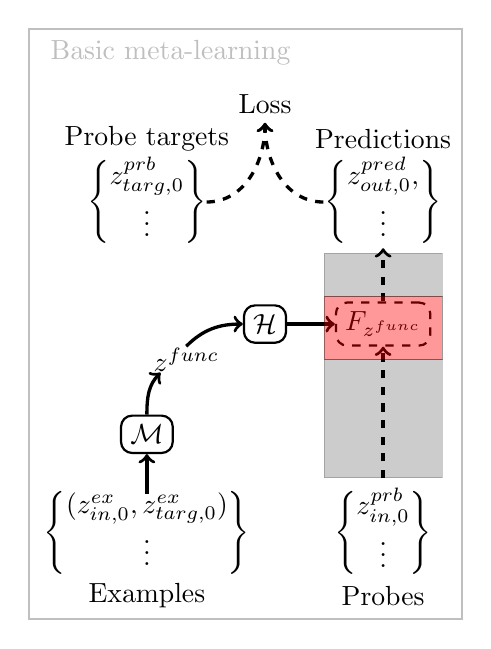
\begin{tikzpicture}
%% basic meta learning
\draw[boundingbox, fill=white] (-3, -4.3) rectangle (2.5, 3.2);
\node[lightgray] at (-1.2, 2.9) {Basic meta-learning};
\node at (-1.5, -4) (examples) {Examples};
\node at (-1.5, -3.2) (D1) {
\(\left\{
\begin{matrix}
(z^{ex}_{in,0}, z^{ex}_{targ,0})\\
$\vdots$
\end{matrix}\right\}\)};

\node at (1.5, -4) (probes) {Probes};
\node at (1.5, -3.2) (D2) {
%\(z^{prb}_{in}\)};
\(\left\{
\begin{matrix}
z^{prb}_{in,0}\\
$\vdots$
\end{matrix}\right\}\)};

\node [block] at (-1.5, -1.95) (M) {\(\mathcal{M}\)};
\path [arrow] ([yshift=-5]D1.north) to (M);

\node at (-1, -1) (zfunc) {\(z^{func}\)};
\path [arrow, out=90, in=-135] (M.north) to ([xshift=6,yshift=3]zfunc.south west);

\node[block] at (0, -0.55) (H) {\(\mathcal{H}\)};
\path [arrow, out=45, in=180] ([yshift=-3]zfunc.north) to (H.west);

\node [block, dashed] at (1.5, -0.55) (F) {\(F_{z^{func}}\)};
\path[arrow] (H.east) to (F.west);

\path [arrow, dashed] (D2) to (F);

\node at (1.5, 1) (outputs) {
%\(z^{pred}_{out}\)};
\(\left\{
\begin{matrix}
z^{pred}_{out,0},\\
$\vdots$
\end{matrix}\right\}\)};
\node at (1.5, 1.8) (predictions) {Predictions};

\path [arrow, dashed] (F) to ([yshift=3]outputs.south);

\node at (-1.5, 1.8) (probetargs) {Probe targets};
\node at (-1.5, 1) (D2targs) {
%\(z^{prb}_{in}\)};
\(\left\{
\begin{matrix}
z^{prb}_{targ,0}\\
$\vdots$
\end{matrix}\right\}\)};

\node [align=center, text width=1.25 cm] at (0, 2.25) (dispatch) {\baselineskip=12pt Loss\par};

\path [arrow, dashed, out=180, in=-90] ([xshift=3]outputs.west) to (dispatch.south);

\path [arrow, dashed, out=0, in=-90] ([xshift=-3.5]D2targs.east) to (dispatch.south);

%% overlay

\draw [fill=black, opacity=0.2] (0.75, -0.2) rectangle (2.25, 0.35);
\draw [fill=red, opacity=0.4] (0.75, -1) rectangle (2.25, -0.2);
\draw [fill=black, opacity=0.2] (0.75, -2.5) rectangle (2.25, -1);

\end{tikzpicture}
\end{column}
\begin{column}{0.5\textwidth}
\includegraphics[width=\textwidth]{figures/poker_function_2.png}
\end{column}
\end{columns}
\end{frame}

\begin{frame}[standout]
We use an architecture which generates task/function-embeddings from examples and uses them to parameterize (part of) a deep network which executes the task. % shorten this
\end{frame}

\section{Homoiconic meta-mapping}

\begin{frame}{Meta-mapping as transforming function embeddings}
* figure here, showing panels a and c from the paper schematic, with a black box in between.
\end{frame}

\begin{frame}{Meta-mapping from examples}
* figure here, repeat figure from meta-mappings are analogous part, replace task reps with embeddings 
\end{frame}

\begin{frame}{Homoiconic meta-mapping architecture}
* figure here, showing full paper schematic (first mask a and c, then show). 
* parsimonious, homoiconic, etc.
\end{frame}

\begin{frame}[standout]
Both basic tasks and meta-mappings can be viewed as functions inferred from examples, so we can use the same approaches and networks for both.
\end{frame}

\begin{frame}{Interim summary}
\begin{itemize}
\item Basic tasks are functions from inputs to outputs (e.g. poker hands to bets), which can be inferred from examples.
\item We represent the task specific computations as relatively simple transformations of an embedding space, parameterized from a task embedding.
\item One type of flexibility is systematically altering these tasks (e.g. trying to bet on losing hands instead of winning ones).
\item This can be seen as a \textbf{meta-mapping}, that is, a function which takes tasks as input and produces tasks as output (e.g. maps try-to-win-at-poker to try-to-lose-at-poker).
\item We implement the meta-mapping function as a transformation of the task embeddings.
\item This function can be learned and implemented using exactly the same networks as the basic tasks.
\end{itemize}
\end{frame}

\section{Experiments}

\begin{frame}{Experiments overview}
This same approach can be used in many different settings: 
\begin{table}
\center
\begin{tabular}{|c|c|c|}
\hline
Experiment & Type & Cognitive motivation \\
\hline
Polynomials & Regression & Proof of concept \\
Card games & Regression & Adapting strategies \\
Categories & Classification & Adapting concepts \\
Grid worlds & RL & Adapting behaviors \\
\hline
\end{tabular}
\end{table}
\end{frame}

\end{document}
